\documentclass[a4paper,10pt]{article}%
\input{commands.tex}%

\usepackage{showkeys}%

\usepackage{stmaryrd}

\usepackage{geometry}

%\title{Segal stuff}%

\usepackage{tikz}%
\tikzset{%
  treenode/.style = {shape=rectangle, rounded corners,%
                     draw, align=center,%
                     top color=white, bottom color=blue!20},%
  root/.style     = {treenode, font=\Large, bottom color=red!30},%
  env/.style      = {treenode, font=\ttfamily\normalsize},%
  dummy/.style    = {circle,draw,inner sep=0pt,minimum size=2mm}%
}%

\usetikzlibrary[decorations.pathreplacing]

\begin{document}		%\maketitle%





\section{Orbital isomorphism sequence does not split}


Let $T \in \Omega_G$
be a $G$-tree and $u(T) \in \Omega$
be the underlying tree of the orbital representation.
Consider the exact sequence
\[
Aut^o_{\Omega_G}(T)
	\to 
Aut_{\Omega_G}(T)
	\xrightarrow{\pi}
Aut_{\Omega}(u(T))	
\]

It is natural to ask if the sequence admits a partial split
$\pi 
\left(
Aut_{\Omega}(u(T))
\right)
\to
Aut_{\Omega_G}(T)
$.

The following example shows it does not.




\begin{example}
Write 
$C_2 = \{\pm 1\}$,
$C_4 = \langle \sigma | \sigma^4 = 1\rangle$,
and set
$G = C_4 \wr C_2
= C_4 \ltimes C_2^{\times 4}$
where the action of 
$C_4$ on $C_2^{\times 4}$
is given by
$\sigma (a,b,c,d) = (d,a,b,c)$.
Set
\[
H = \{(\pm 1, 1 ,\pm 1, 1)\}
\qquad
K = C_2^{\times 4} = \{(\pm 1, \pm 1 ,\pm 1, \pm 1)\}
\]
and consider the $G$-tree
\[
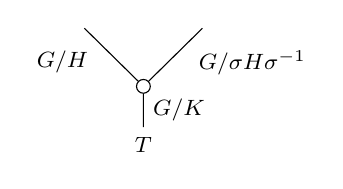
\begin{tikzpicture}[grow=up,auto,level distance=2.1em,every node/.style = {font=\footnotesize},dummy/.style={circle,draw,inner sep=0pt,minimum size=1.75mm}]
\node at (-2,-1) {$T$}
child{node [dummy] {}
	child{
		edge from parent node [swap,near end] {$G/ \sigma H\sigma^{-1}$}}
	child{
		edge from parent node[near end] {$G/H$}}
	edge from parent node [swap] {$G/K$}};
\end{tikzpicture}
\]
The tree $T$ has an automorphism
described by
\begin{equation}\label{AUTO EQ}
	G/H \xrightarrow{\sigma} G/ \sigma H\sigma^{-1}
\qquad
	G/ \sigma H\sigma^{-1} \xrightarrow{\sigma} G/H
\qquad
	G/K \xrightarrow{\sigma} G/K 
\end{equation}
which determines an element of order $2$ in 
$Aut_{\Omega}(u(T))$.
However,  
\eqref{AUTO EQ}
does not have order $2$, 
and likewise for any other possible lift, 
which must have either the form
\begin{equation}
G/H \xrightarrow{\sigma k } G/ \sigma H\sigma^{-1}
\qquad
G/ \sigma H\sigma^{-1} \xrightarrow{\sigma \bar{k}} G/H
\qquad
G/K \xrightarrow{\sigma} G/K 
\end{equation}
or
\begin{equation}
G/H \xrightarrow{\sigma^{\-1} k } G/ \sigma H\sigma^{-1}
\qquad
G/ \sigma H\sigma^{-1} \xrightarrow{\sigma^{-1} \bar{k}} G/H
\qquad
G/K \xrightarrow{\sigma^{-1}} G/K 
\end{equation}
for some $k,\bar{k}$ of the form $(1,\pm 1, 1, \pm 1)$.
\end{example}	














\newpage

\bibliography{biblio}{}



\bibliographystyle{abbrv}



\end{document}